\graphicspath{{figures/chapter3/}}
\onehalfspacing

\chapter{UAV photogrammetry for annual glacier reconstruction (2015-2023)}\label{ch:3}

\vfill

\newthought{This chapter is based on:}

\begin{itemize}
    \item \noindent Ioli, F., Bianchi, A., Cina, A., De Michele, C., Maschio, P., Passoni, D., \&
Pinto, L. (2021). Mid-Term Monitoring of Glacier’s Variations with UAVs: The Example of the Belvedere Glacier. Remote Sensing, 14(1), 28. \url{https://doi.org/10.3390/rs14010028}
    \item Ioli, F., De Gaetani, C., Barbieri, F., Gaspari, F., Pinto, L., \& Rossi, L. (2024). Belvedere Glacier long-term monitoring Open Data [Data set]. Zenodo. \url{https://zenodo.org/doi/10.5281/zenodo.7842347}
\end{itemize}

\newpage

\section{Introduction}\label{sec:3:intro}

This chapter investigates the potential of high-resolution UAV photogrammetry and in-situ GNSS measurements for comprehensive monitoring of the Belvedere Glacier. 
Originally, our understanding of glacier dynamics has been constrained by the limitations of traditional aerial photogrammetry, which provided data at approximately decadal intervals and sub-meter resolution. 
A UAV-based approach offers a paradigm shift, enabling annual reconstructions with sub-decimeter resolution.
With this enhanced capability, we can delve into the yearly kinematics of the glacier, gaining deeper insights into its evolution and responses to climate change.

Started in 2015, the Belvedere Glacier monitoring campaign was designed and conducted jointly by the Department of Civil and Environmental Engineering (DICA) of Politecnico di Milano and the Department of Environment, Land and Infrastructure Engineering (DIATI) of Politecnico di Torino. 
Moreover, the DREAM projects (DRone tEchnnology for wAter resources and hydrologic hazard Monitoring), involving teachers and students from Alta Scuola Politecnica (ASP) of Politecnico di Torino and Milano, contributed to the campaign from 2015 to 2017.

Every year, fixed-wing UAVs and quadcopters were used to remotely sense the glacier and build high-resolution 3D photogrammetric models, DSMs, and orthophotos.
The series of point clouds was used to estimate the glacier volume variations and estimate the thinning of the glacier.
Additionally, the orthophotos and the DSMs were used to investigate the glacier kinematics and derive ice flow velocity and glacier retreat. 
This was carried out by exploiting DIC techniques to track the movement of the glacier surface.

The Belvedere Glacier monitoring campaign has produced a rich dataset of GNSS measurements, 3D point clouds, DSMs, and orthophotos. 
Recognizing the transformative potential of open science, we have made this entire dataset publicly available through a Zenodo repository\footnote{\url{https://zenodo.org/doi/10.5281/zenodo.7842347}}.
To facilitate the management and accessibility of the data, we have implemented a PostgreSQL relational database to store and manage key survey data, measurement outcomes, and derived products. 
Additionally, we have also developed a suite of web-based tools to make the data user-friendly for researchers and non-experts\footnote{\url{https://thebelvedereglacier.it/}}.
This includes a Potree-based platform \citep{schutz2016potree}, which allows users to explore the glacier models through any web browser, navigate across different survey years, and directly visualize the glacier's evolution over time.
This chapter will finally describe the set of solutions to promote the widespread use of our monitoring data, accelerating scientific progress in glacier research and encouraging knowledge sharing across the scientific community.

\section{Instruments and datasets}\label{sec:3:instrument}
 
This section introduces the data acquired in this study from 2015 to 2023, including the periodical GNSS measurements of targets deployed over the glacier and UAV images acquired to build the photogrammetric reconstructions.

\subsection{GNSS measurements}\label{sec:3:gnss}

Yearly GNSS measurements of permanent targets deployed across the glacier were conducted. 
These targets served a dual purpose: as GCPs/CPs for photogrammetric block processing and as high-accuracy 
reference points for evaluating glacier kinematics derived from photogrammetry. 
The targets were materialized using square cross patterns printed on polypropylene sheets and anchored to 
large rocks and boulders (\figref{fig:3:belvedereGCP}b).
Approximately 25 targets were deployed on the glacier itself (designated as as \textit{moving targets} or 
\textit{M\#} in \figref{fig:3:belvedereGCP}a), while 24 targets were placed on stable areas along the moraines 
(labelled as \textit{stable targets} or \textit{S\#} in \figref{fig:3:belvedereGCP}a). 

Annually, we evaluated the condition of each target. Damaged or destroyed targets were replaced with new polypropylene plates, maintaining the original center location using the existing plugs. 
Over time, some targets were lost and replaced with new ones positioned near the original locations (e.g., M29bis).

All targets were surveyed with dual frequency geodetic quality GNSS receivers: 
Leica GPS VivaGS14 and Leica GPS1200+.
The measurements were framed within the official Italian reference system ETRF2000
at the epoch 2008.0, projected in UTM 32N (RDN2008 / UTM zone 32N, EPSG:7791).
The measurement techniques employed in the survey have evolved over time.
Before 2021, target positions on the lower glacier (where GSM network coverage was available) 
were determined using nRTK relative to CORS permanent stations (either HxGN SmartNet or SPIN GNSS).
These points were occupied for at least two 5-second intervals. 
In contrast, upper glacier targets were surveyed using static sessions of approximately 10 
minutes, with raw data post-processed relative to local master stations located in stable areas 
(S12 or S20, see \figref{fig:3:belvedereGCP}a).
Since 2021, GNSS measurements were conducted in RTK mode using a local base station 
(\textit{S12} or \textit{S20}).
The real-time corrections were streamed from the base to the rover by a radio link connection. 
his approach has significantly reduced measurement time in the upper glacier, requiring seconds 
rather than minutes per occupation, as was for static processing.
Additionally, the local-base RTK method improves internal coherence among measurements, 
as well as tropospheric and ionospheric error modeling due to shorter baselines compared to 
the nRTK approach.

The accuracy of GNSS measurements was evaluated empirically by comparing repeated
measurements over stable targets carried out in different years.
RMSE of \qty{1.5}{\centi\meter} in planimetry and \qty{3}{\centi\meter} in elevation were
obtained.

\begin{figure}
    \centering
    \subcaptionbox{\label{fig:3:studyarea:map}}{
        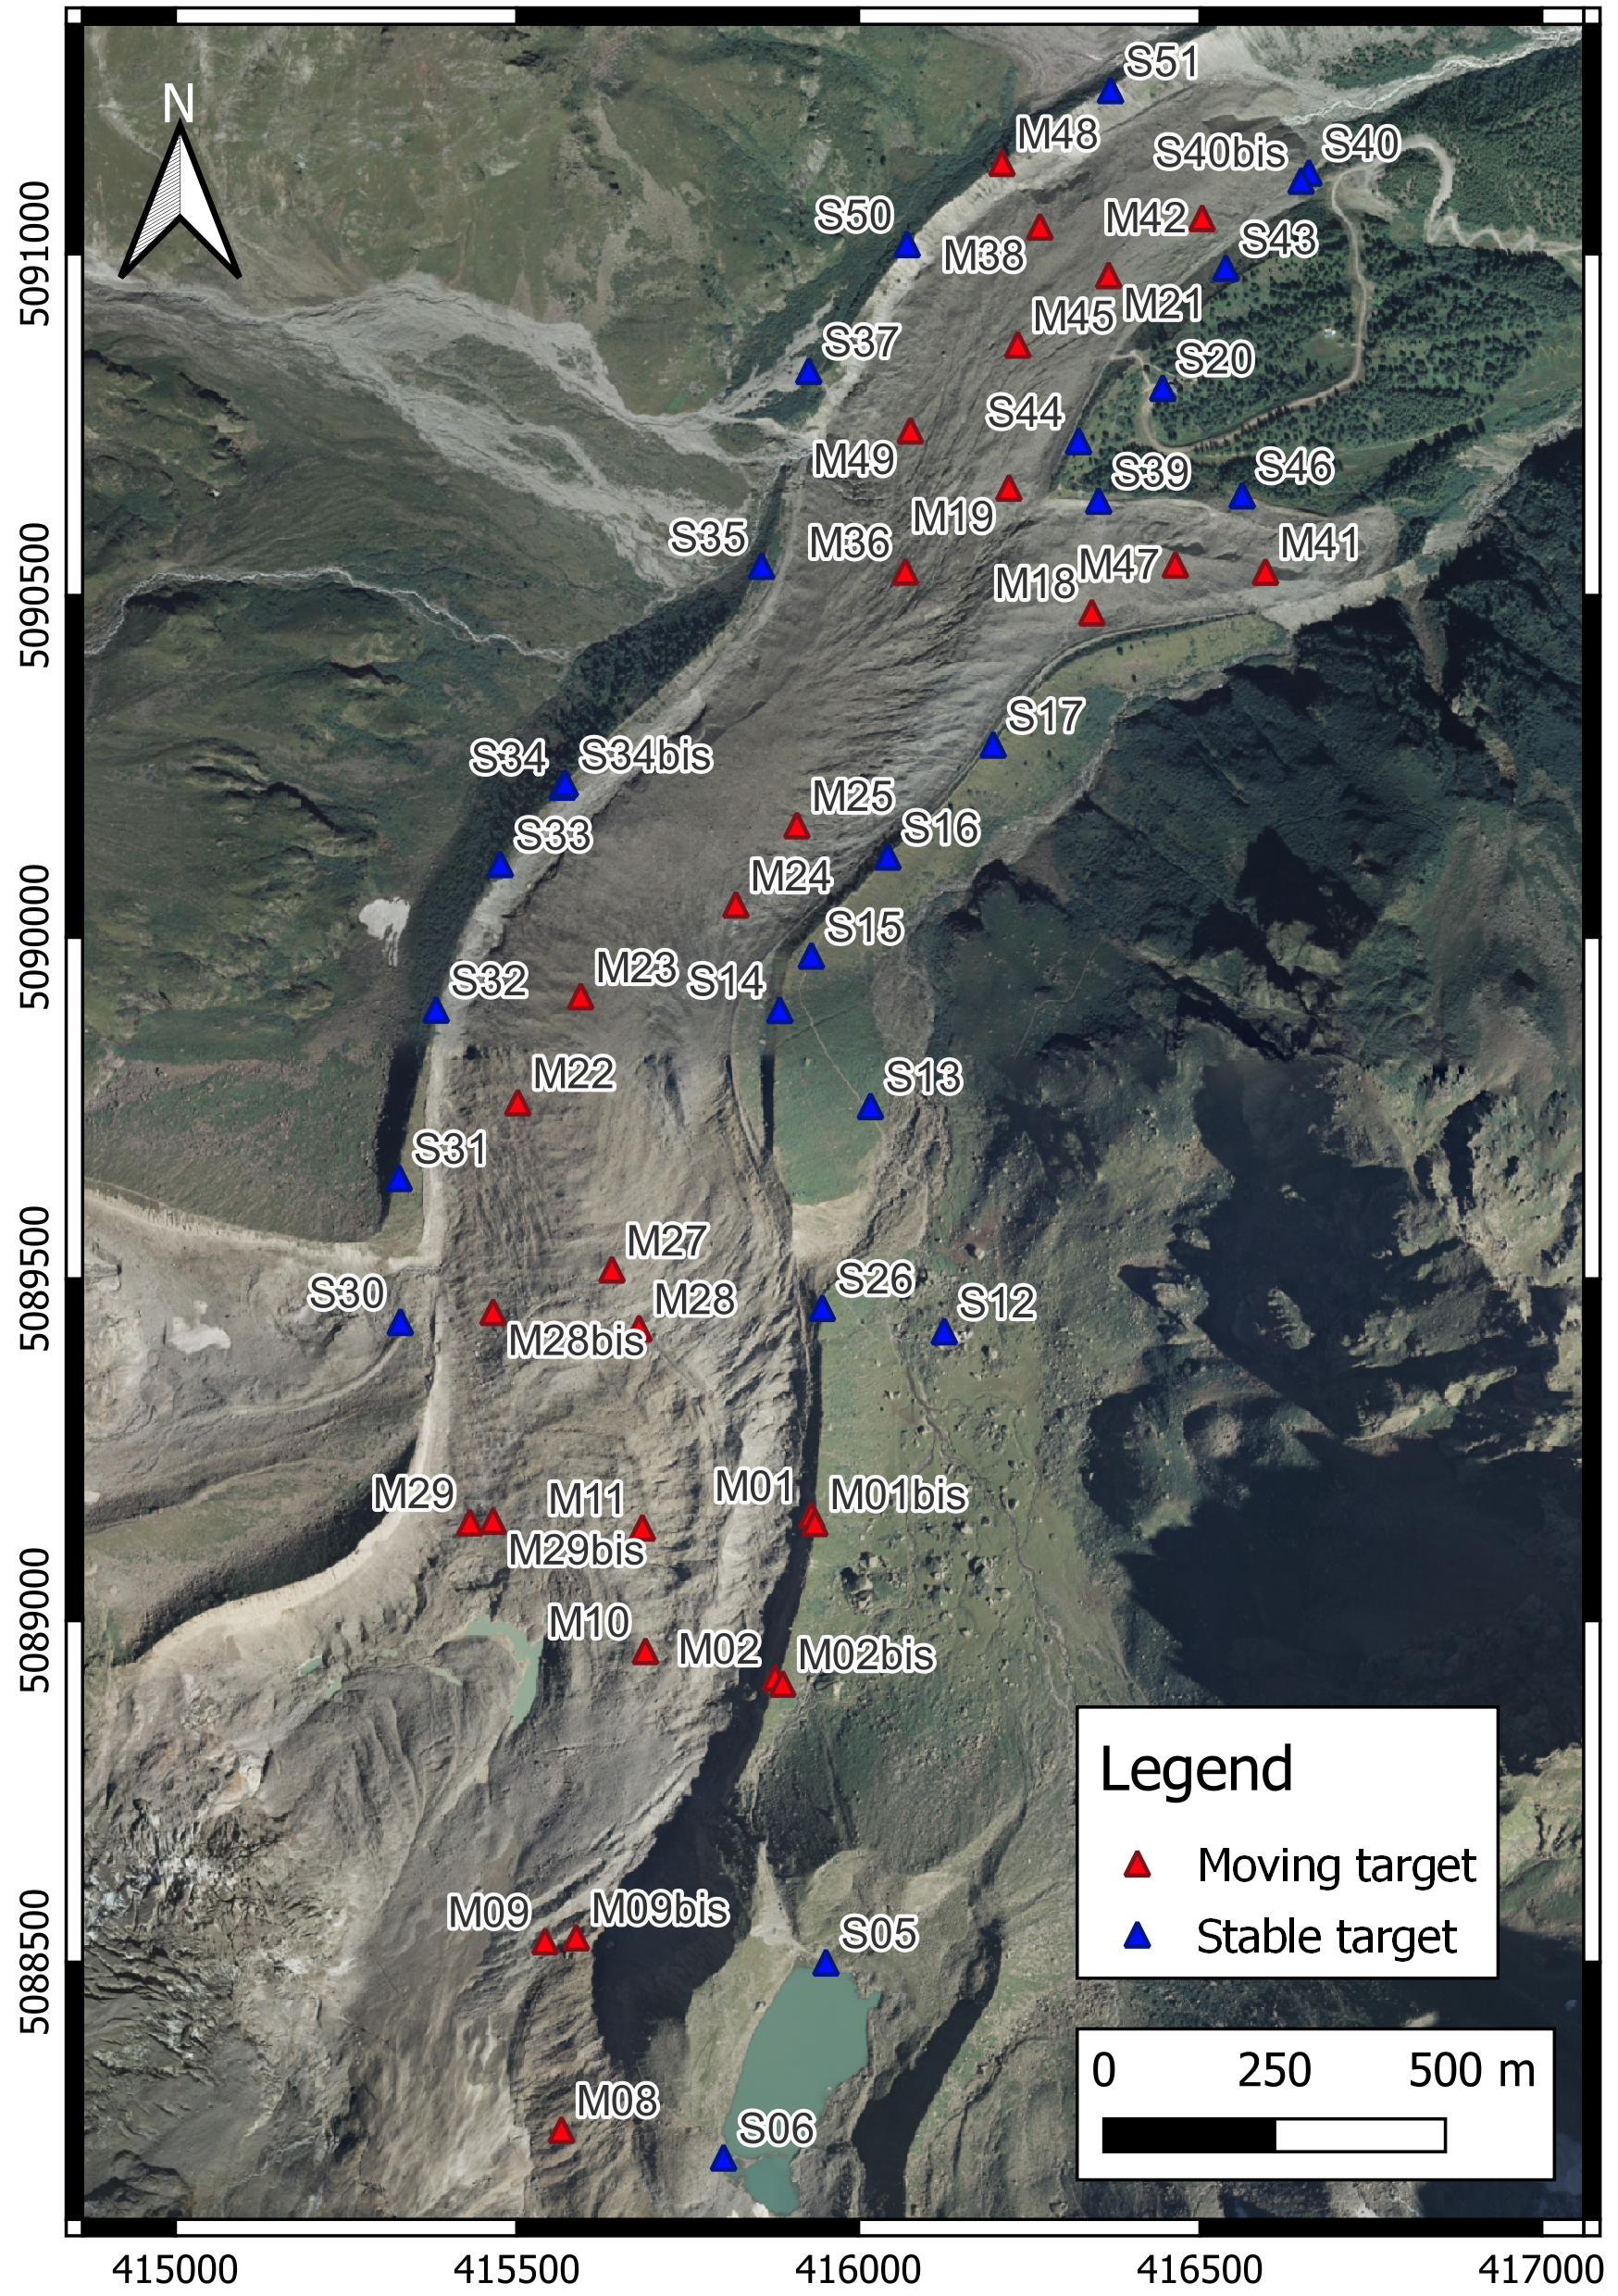
\includegraphics[width=.6\textwidth]{belvedereGCP.png}
    }
    \subcaptionbox{\label{fig:3:studyarea:pic}}{
        \includegraphics[width=.35\textwidth]{target.jpg}
    }
    \caption{(\textbf{a}) Location of the targets used for the
        photogrammetric surveys. For~each year, a~subset of the targets were used as GCPs, while the remaining as~CPs; (\textbf{b}) an example of a photogrammetric target deployed over the glacier moraine.}
    \label{fig:3:belvedereGCP}
\end{figure}

\subsection{UAV flights}\label{sec:3:uav-flights}

The long duration of the monitoring campaign, challenging environment, and involvement of 
multiple research groups led to the use of various UAV platforms and cameras over time. 
\tabref{tab:3:datasets} provides a detailed summary of the equipment (UAV and camera) employed, while 
\tabref{tab:3:camere} lists the main sensor and lens specifications for each camera.

In 2015 and 2016, a ready-to-fly fixed-wing SenseFly eBee equipped with a compact camera Canon
PowerShot S110 was used for whole glacier surveys.
Due to technical problems, the year 2017 saw the use of different UAVs (both fixed-wing and quadcopters)
and camera combinations (\tabref{tab:3:datasets}). 
From 2018 to 2020, a low-cost recreational Parrot Disco FPV fixed-wing UAV (wingspan 1.15 m, weight 750 g) 
was adapted to carry a lightweight Hawkeye Firefly 8S action camera.

In 2021, a professional-grade DJI Matrice 210 V2 quadcopter was employed, carrying a 
DJI ZenMuse X5s camera featuring a Micro 4/3 sensor and a 15 mm lens. 
Since 2022, the UAV platform has been upgraded to a DJI Matrice 300 RTK quadcopter
paired with a full-frame DJI Zenmuse P1 camera and a DL 35 mm F2.8 LS ASPH lens.
While this setup offered superior image quality, the longer focal length necessitates 
higher flight altitudes to maintain a consistent GSD with the previous surveys.
Furthermore, the DJI Matrice 300 RTK was equipped with an RTK GNSS receiver, enabling 
decimeter-level accuracy in recording the camera position for each shot. 
This precision was achieved through a local GNSS base station positioned near the take-off 
location, which streamed real-time corrections to the drone via DJI's proprietary link.

UAV flights were conducted automatically by using ground station software packages
developed by UAV manufacturers and UgCS\footnote{\url{https://www.sphengineering.com/flight-planning/ugcs}}
flight planning software.
The flights were designed to have GSD ranging between \qtylist{5;10}{\centi\meter}, and
to guarantee \qty{\sim 80}{\percent} of longitudinal and \qty{\sim 60}{\percent} of
transversal overlap.
Average image GSD values and number of GCPs and CPs, used respectively to orient the
images and to assess the quality of the photogrammetric blocks, are summarized in
\tabref{tab:3:datasets}.

\begin{table}[p]
    \small
    \centering
    \caption{Summary of the characteristics of the surveys.}
    \begin{tabular}{c  m{1.8cm} m{3.5cm} m{4.2cm} c c c }
        \toprule
        Year                                                              & Date
                                                                          & UAV
                                                                          & Camera
                                                                          & GSD
                                                                          & GCP
                                                                          & CP
        \\
                                                                          &
                                                                          &
                                                                          &
                                                                          & [m/px]
                                                                          & [\#]
                                                                          & [\#]
        \\
        \midrule
        2015                                                              & A.
        8.10\newline B. 23.10                                             &
        SenseFly eBee                                                     & Canon
        PowerShot S110                                                    & 0.07
                                                                          & 24
                                                                          & 11
        \\[4mm]
        2016                                                              & 20.10
                                                                          & SenseFly eBee
                                                                          & Canon
        PowerShot S110                                                    & 0.09
                                                                          & 31
                                                                          &
        15
        \\[4mm]
        2017                                                              & A.
        5.10\newline B. 15.11\newline C. 16.11                            & A. SenseFly
        eBee \newline B. SenseFly eBee Plus\newline  C. DJI Phantom 4 Pro & A. Canon
        PowerShot
        S110  \newline B. SenseFly S.O.D.A \newline C. DJI FC6310         & 0.06
                                                                          & 27
                                                                          & 8
        \\[4mm]
        2018                                                              & 23-25.07
                                                                          & Parrot Disco
                                                                          & Hawkeye
        Firefly 8S                                                        & 0.05
                                                                          & 27
                                                                          &
        13
        \\[4mm]
        2019                                                              & 29.07-2.08
                                                                          & Parrot Disco
                                                                          & Hawkeye
        Firefly 8S                                                        & 0.06
                                                                          & 26
                                                                          &
        10
        \\[4mm]
        2020                                                              & A. 26-27.07
        \newline B. 9.08                                                  & A.
        Parrot Disco\newline B. DJI Phantom 4 Pro                         & A. Hawkeye
        Firefly 8S\newline B. DJI FC6310                                  &
        0.05                                                              & 29
                                                                          & 12
        \\[4mm]
        2021                                                              & 29.07-2.08
                                                                          & DJI Matrice 210 V2
                                                                          & DJI ZenMuse x5s
                                                                          & 0.04
                                                                          & 23
                                                                          &
        9
        \\[4mm]        
        2022                                                              & 28.07-29.07
                                                                          & DJI Matrice 300 RTK
                                                                          & DJI Zenmuse P1 - 35 mm
                                                                          & 0.03
                                                                          & 22
                                                                          &
        19
        \\[4mm]
        2023                                                              & 25.07-27.07
                                                                          & DJI Matrice 300 RTK
                                                                          & DJI Zenmuse P1 - 35 mm
                                                                          & 0.03
                                                                          & 23
                                                                          &
        9
        \\[4mm]        
        \bottomrule

    \end{tabular}
    \label{tab:3:datasets}
\end{table}

\begin{table}[p]
    \centering
    \small
    \caption{Summary of the characteristics of the cameras employed.}
    \begin{tabular}{c c c c c c}
        \toprule
        Camera                        & Sensor                        & Sensor Size
                                      & Focal length                  & Image size
                                      & Pixel size
        \\
                                      &                               &
        [\SI{}{\milli\meter\squared}] & \newline[\SI{}{\milli\meter}] & [\SI{}{\pixel}]
                                      & \newline[\SI{}{\micro\meter}]
        \\

        \midrule
        Canon PowerShot S110          & 1/1.7" CMOS                   & $7.44\times5.58$
                                      & 5.2                           & $ 4000 \times
            3000
        $                             & 1.9
        \\
        SenseFly S.O.D.A              & 1" CCD                        & $13.2\times8.8$
                                      & 10.6                          & $5472 \times
        3648$                         & 2.4
        \\
        DJI FC6310                    & 1" CMOS                       & $13.2\times8.8$
                                      & 8.8                           & $5472 \times3648$
                                      & 2.4
        \\
        Hawkeye Firefly 8S            & 1/2.3" CMOS                   & $6.17\times4.56$
                                      & 3.8                           & $5472 \times3648$
                                      &
        1.34
        \\
        DJI ZenMuse x5s               & 4/3" CMOS                     & $17.3\times13$
                                      & 15                            & $5280 \times
        3956$                         & 3.3 
        \\
        DJI Zenmuse P1 - 35 mm        & FullFrame CMOS                & $35.9\times24$
                                      & 35                            & $8192 \times
        5460$                         & 4.4
        \\
        \bottomrule
    \end{tabular}
    \label{tab:3:camere}
\end{table}

\subsection{Challenges and adaptations in the 2017, 2018 and 2020 surveys}\label{sec:3:problems} 

Conducting annual monitoring campaigns in alpine environments poses logistical and environmental
challenges, including limited accessibility in certain areas and unpredictable weather. 
These factors directly impacted the 2017 and 2020 surveys.

Adverse weather and logistical constraints necessitated splitting the 2017 survey across 
multiple dates, requiring using different UAVs and cameras (see \tabref{tab:3:datasets}). 
Consequently, the photogrammetric model was built in three parts. 
The central portion corresponds to a survey carried out in October, while the snow-covered 
upper and lower sections were acquired in November (\figref{fig:3:ortophoto}c).

Technical issues arose during the 2020 survey when an elevon servo failed during landing and
caused the fixed-wing UAV to crash.
To complete the survey, a DJI Phantom 4 Pro quadcopter was employed 14 days later to survey 
the upper part of the glacier (see the different colors in the orthophoto of
\figref{fig:3:ortophoto}f).
However, the harsh terrain and the presence of crevasses in the upper part of the glacier 
prevented the measurement of additional GCPs to constrain the model in this region. 
This necessitated co-registering the Phantom 4 Pro model with the 2019 data, 
using stable rock features along the moraines as reference points. 
This approach was less accurate than measuring GCPs directly on the field and yielded an
RMSE on CPs of \SI{0.36}{\meter} (see \figref{fig:3:CP_errors}), \SI{\sim 7}{}~times the GSD.
Nevertheless, the area affected by this problem consisted of the upper accumulation area only
and it was rather limited compared to the whole Belvedere~Glacier.

The project timeline also led to a shift in survey periods from autumn (2015-2017) 
to summer (2018-2023).
This change means that the timespan between the October/November 2017 and July 2018 
surveys does not encompass the summer (neither August 2017 nor August 2018 was included), 
which is the period of maximum glacier ablation and surface velocity. 
Consequently, volume variation and ice flow velocity estimated between 2017 and 2018 reflect
primarily winter conditions and are not directly comparable to other years, as they underestimate
the actual annual average statistics.

\section{Metodology}\label{sec:3:methodology}

\subsection{SfM workflow}\label{sec:3:sfm}

To generate photogrammetric models of the glacier, UAV imagery was processed using 
Agisoft Metashape 1.8.5\footnote{\url{https://www.agisoft.com}}.
Each year, a minimum of 22 GCPs distributed across the glacier were used for image 
orientation, while at least 8 CPs served for model quality assessment.  
All GCPs and CPs were manually collimated within the images.

Tie Points (TPs) were detected and matched by Metashape on full-resolution images (which
corresponds to \textit{high accuracy} parameter in Metashape).
Image External Orientation (EO) and TPs world coordinates were estimated by solving the
Bundle Block Adjustment (BBA).
TPs with the worst reprojection error on images were removed and the BBA was solved again to improve the quality of the solution.
This process was iterated more times until the TP mean reprojection error had dropped below
\SI{\sim 0.8}{\pixel}.
Camera internal orientation was estimated by self-calibration
\citep{Fraser2013, Cramer2017}, because of its instability in the cameras employed.

Agisoft Metashape computed dense 3D reconstruction with proprietary MVS
algorithms~\citep{Dallasta}.
Depth maps and dense point clouds were obtained from images downsampled by a factor of 4, in~order to reduce the computational time (\textit{medium quality} parameter of the dense cloud generation in Metashape).
Triangulated mesh surfaces and photorealistic textures were computed.

DSMs with a resolution of \SI{0.5}{\meter\per\pixel} were derived from the mesh model.
Finally, orthophotos with a GSD of \SI{0.10}{\meter\per\pixel} were obtained by
projecting the most nadiral images over the mesh model.

\subsection{Glacier flow velocity}\label{sec:3:method_velocity}

In debris-covered glaciers, surface debris and boulders primarily move in conjunction with the underlying ice flow, making them valuable proxies for evaluating glacier kinematics through tracking techniques~\citep{Dehecq2015, Sam2016, Blothe2021}.

In-situ GNSS measurements of the \textit{moving targets} anchored to large rocks (see~\secref{sec:3:gnss}) were used as a method for deriving glacier surface flow velocities.
These punctual measurements, labeled as \textit{GNSS}, provided high-accuracy, 
estimated at approximately \qty{\sim 3}{\centi\meter} (see Section~\ref{sec:3:gnss}).
Assuming measurements of the same target at two consecutive years as independent, the expected standard deviation 
of the velocity was computed by propagating the variance as \qty{\pm 0.04}{\meter\per\year}.
Therefore, GNSS measurements were considered the most reliable reference for flow velocity estimation.
However, due to the limited number of GNSS measurement points across the glacier, they are insufficient 
for deriving a complete glacier velocity field.

To derive a complete description of the surface kinematics, DIC algorithms was employed. 
From 2018 onwards, consistent acquisition periods (end of July) and snow-free conditions enabled the use of DIC on UAV orthophotos for comprehensive velocity field derivation.
On the other hand, the presence of snow and significant environmental variations between orthophotos from 2015 to 2018
(\figref{fig:3:ortophoto}) made them unsuitable for DIC techniques.
Consequently, we applied DIC on pairs of DSMs \citep{Gindraux2019} to extract glacier surface displacements for this period.
% Additionally, we manually tracked characteristic features (e.g., sharp edges of large rocks) across multiple orthophotos 
% \citep{Lucchitta1986} to derive velocity fields (we refer to these points as MAN).

To compute displacement by DIC, we employed the open-source Local Adaptive Multiscale Image Matching Algorithm (LAMMA)~\citep{Dematteis2022}.
LAMMA adopts a hierarchy structure of patch grids of increasing spatial resolution and uses locally-adaptive search area sizes, according to the displacements already
obtained in the neighboring region.
Lamma was originally written in Matlab\footnote{\url{https://github.com/niccolodematteis/LAMMA}}, but we have 
recently translated it into Python for multitemporal processing of stereo images \citep{ioli2024deep} and 
published it as an open-source library, named pyLamma\footnote{\url{https://github.com/franioli/pylamma/}}.

As a correlation function, we used the cosine similarity applied to orientation images \citep{Dematteis2021}, 
which is less sensitive to chromatic variation changes (e.g., due to to shadows or snow patterns) and is known 
to perform well in glacier environments \citep{Heid2012_evaluation_xcorr, Dematteis2019}.
The cosine similarity function is defined as \citep{Dematteis2022}:
\begin{equation}
\text{CXC}(r,c) = \frac{1}{RC} \sum_{r,c} \mathrm{Re} \left( A_{\text{or}}^{*}(i,j) \cdot B_{\text{or}}(i+r,j+c) \right)
\end{equation}
where $A_{or}$ and $B_{or}$ denotes the complex conjugate and are the orientation images of the 
reference and slave patches, respectively. 
An orientation image is defined as $ I_{\text{or}} = \frac{I_x}{|I_x|} + i\frac{I_y}{|I_y|} $, 
where are the first derivatives of the image intensity in the two dimensions \citep{fitch2002_OC}.

All image pairs processed with pyLamma (DSM pairs for 2015-2018, and orthophotos from 2019-2023) maintained a 
consistent ground resolution of \SI{0.2}{\meter\per\pixel}. 
To analyze these images, we established a regular grid of nodes spaced \SI{64}{\pixel} apart (equivalent to \SI{12.8}{\meter} 
on the ground).
The interrogation area (i.e., the size of the template defined around each node in the master image that is searched in the slave image)
was set to the same size as the grid step.
This was empirically chosen as a trade-off to balance a stronger correlation peak (achieved with a larger area used to 
compute the correlation function) with maintaining similar kinematics within the interrogation area, as an excessively 
large area risks including regions with different kinematics, potentially weakening the results. 
We employed pyLamma's multi-scale processing with a 3-step scale approach to optimize the interrogation area hierarchically.  
This strategy involved starting the displacement calculation at a coarser scale, using an interrogation area of \SI{256}{\pixel}. 
This provided an initial displacement estimate, which we leveraged to refine the search area at finer scales.  
We based the initial interrogation area size on expected minimum and maximum glacier displacements derived from GNSS measurements, 
ensuring our analysis was tailored to the specific glacier's movement.

To achieve subpixel displacement sensitivity, LAMMA considers the sub-region of the similarity function centred 
in its maximum value and it oversamples this sub-region using bicubic interpolation \citep{Dematteis2022}.
Then, the subpixel displacement is the peak's position of the oversampled correlation function \citep{Debella_Gilo2011}.
We used an upsampling factor of 10 to upsample the correlation function. 

% Assuming collimation standard deviation of \SI{\sim 2}{\pixel} and considering the planimetric accuracy of 
% the orthophotos of \SI{\sim 0.1}{\meter} (Figure~\ref{fig:3:CP_errors}), 
% the~standard deviation of the velocity obtained from MAN points was estimated as \SI{\pm 0.3}{m/y} 
% by variance propagation (covariances were neglected, assuming the orthophotos as independent).  

% While less precise than DIC, manual selection by a human operator ensured high matching reliability. 
% To maintain uniform distribution, features were selected on a \qtyproduct{100 x 100}{\metre} grid whenever possible, resulting 
% in approximately 130 points (with approximately (approximately one point every \qty{10000}{\meter\squared})).  
% Unfortunately, some points were lost over time, leaving only 115 identifiable on the 2020 orthophoto.

\subsection{Volume variations}\label{sec:3:method_volumes}

To compute glacier volume variation $ \Delta V $, consecutive DSMs were differentiated
by employing a DEM of Difference (DOD) approach.
To this end, the tool \textit{Compute 2.5D volume} implemented in 
CloudCompare~\footnote{Cloudcompare: \url{https://www.danielgm.net/cc/}} was used.
First, photogrammetric dense clouds were gridded by projecting points along the vertical
direction onto a planar surface, resulting in DSMs with a \qtyproduct{0.5x0.5}{\meter} ground resolution.
This resolution balances robust height estimation (by averaging a sufficient number of points per cell) 
with the ability to resolve finer-scale glacier morphology.
A manually created mask delineated the glacier surface within each DSM, ensuring only 
relevant areas were analyzed.  
DSMs from consecutive years were then subtracted pixel-by-pixel, yielding the height 
difference for each raster cell.

A simplified approach was initially used to estimate volume variation variance, 
treating each DSM as a mono-dimensional random variable with variance equal to the squared 
vertical RMSE computed on CPs.  
While providing a preliminary idea, a more rigorous uncertainty estimation would require 
several additional considerations.
Firstly, to propagate variance accurately, we need the full covariance matrix of each DSM. 
This information is not provided by the SfM software (Agisoft Metashape), hindering the 
calculation of covariances between neighboring DSM cells (which are correlated due to 
shared image sources).
Additionally, the available 3x3 covariance matrices from the sparse point cloud reflect
bundle adjustment errors but may not capture systematic biases like the doming 
effect~\citep{James2014_mitigating, James2020_mitigating2}.
Finally, these variances pertain only to the sparse point cloud and would require 
interpolation onto the DSM grid.
A potential solution for more robust DSM covariance estimation lies in Monte Carlo simulations, 
as carried out by \citet{James2017_3duncertainty} and \citet{Roncella2021_montecarlo}.

Consequently, due to these limitations, we derived a rough variance estimation by
assuming a constant variance of the DSM equal to the squared vertical RMSE computed on CPs.
Assuming DSMs computed at different years as independent, the volume variation variance 
was calculated as follows:
\begin{equation}
    \sigma^2_{\Delta V^{(i+1,i)}}  = {(n \times A_c)}^2 \left( \sigma^2
    _{DSM^{(i+1)}} + \sigma^2_{DSM^{(i)}} \right),
    \label{eq:3:volVarProp}
\end{equation}
where $ n $ is the number of cell in the~DSMs, $A_c$ is the area of the cells
and $ \sigma^2 _{DSM}$ is the squared vertical error of the photogrammetric model.

Between 2015 and 2018, the partial snow cover (\figref{fig:3:ortophoto}a--c)) introduced
additional uncertainty in volume estimation. 
To address this, snow depth data measured from the meteorological station located close 
to the Zamboni Zappa 
Hut\footnote{\mbox{\url{https://www.arpa.piemonte.it/rischinaturali/accesso-ai-dati/annali_meteoidrologici/annali-meteo-idro/banca-dati-meteorologica.html}}} 
was used as a first estimate of the snow depth for the upper part of the glacier. 
The snow depths measured on survey dates are the following
\begin{itemize}
    \item 2015 (Oct. 23): 22 cm
    \item 2016 (Oct. 20): 20 cm
    \item 2017 (Nov. 15): 40 cm
\end{itemize}
These depths were incorporated into the DSM standard deviations. 
However, due to the partial snow cover, the snow-driven uncertainty was weighted 
by half the total glacier area during variance propagation.

\section{Results}\label{sec:3:res}

\subsection{SfM}\label{sec:3:res:sfm}

\begin{figure}[ht!]
    \centering
    \includegraphics[width=0.9\columnwidth]{uav_cp_error.png}
    \caption{Barplot of reprojection RMSE computed on CPs for each photogrammetric
        model. Due to the technical problems that occurred in 2020 
        (see \secref{sec:3:problems}), the 2020 RMSE refers only to the survey of
        the lower part of the glacier, excluding the upper accumulation sector.
    }
    \label{fig:3:CP_errors}
\end{figure}

\begin{figure}
    \centering
    \subcaptionbox{\label{fig:3:ortophoto:2015}}{
        \includegraphics[width=0.25\textwidth]{orto2015.jpg}
    }
    \subcaptionbox{\label{fig:3:ortophoto:2016}}{
        \includegraphics[width=0.25\textwidth]{orto2016.jpg}
    }
    \subcaptionbox{\label{fig:3:ortophoto:2017}}{
        \includegraphics[width=0.25\textwidth]{orto2017.jpg}
    }
    \\
    \subcaptionbox{\label{fig:3:ortophoto:2018}}{
        \includegraphics[width=0.25\textwidth]{orto2018.jpg}
    }
    \subcaptionbox{\label{fig:3:ortophoto:2019}}{
        \includegraphics[width=0.25\textwidth]{orto2019.jpg}
    }
    \subcaptionbox{\label{fig:3:ortophoto:2020}}{
        \includegraphics[width=0.25\textwidth]{orto2020.jpg}
    }
    \subcaptionbox{\label{fig:3:ortophoto:2021}}{
        \includegraphics[width=0.25\textwidth]{orto2021.jpg}
    }
    \subcaptionbox{\label{fig:3:ortophoto:2022}}{
        \includegraphics[width=0.25\textwidth]{orto2022.jpg}
    }
    \subcaptionbox{\label{fig:3:ortophoto:2023}}{
        \includegraphics[width=0.25\textwidth]{orto2023.jpg}
    }
    \caption{Orthophotos obtained from the photogrammetric model for each year.
        (\textbf{a}) 2015, (\textbf{b}) 2016, (\textbf{c}) 2017, (\textbf{d}) 2018,
        (\textbf{e}) 2019, (\textbf{f}) 2020, (\textbf{g}) 2021, (\textbf{h}) 2022, (\textbf{i})
        2023. All the orthophotos are in 1:25000 scale and they are overlapped to the Swisstopo base-map (source: Swisstopo
        www.geo.admin.ch)}
    \label{fig:3:ortophoto}
\end{figure}

Each SfM process yielded a 3D point cloud, a textured mesh, a DSM, and an orthophoto of the glacier. 
Point cloud density increased over time: point clouds from 2015 to 2020 contained \SI{0.5e8}{} to \SI{1e8}{} 
points, while those from 2021 onwards had \SI{1.5e8}{} to \SI{2.5e8}{} points. 
DSMs and orthophotos were produced at a resolution of 20 centimeters per pixel 
Due to autumn surveys, orthophotos from 2015 to 2017 show some snow cover (\figref{fig:3:ortophoto}).

The geometrical accuracy of the SfM models was evaluated for all years using CPs.
\figref{fig:3:CP_errors} RMSE of on-ground error in all three directions and globally. 
RMSE values range between 0.1 and 0.2 meters across all components and years. 
Note that for 2020, errors only reflect the lower part of the glacier. 
The upper part was sensed with a separate photogrammetric flight that lacked GNSS-measured
GCPs and instead relied on natural features identified in the 2019 model as GCPs (see \secref{sec:3:problems}).

% From 2015 to 2017, when compact cameras were used, errors smaller than 2 times the GSD
% were obtained.
% From 2018 to 2020, a lightweight action-cam has been employed to minimize the UAV take-off
% weight and this has led to an RMSE up to 3~times the GSD, but~still always smaller than
% \SI{0.2}{\meter}.
% From 2021, errors smaller than 2 times the GSD
% accuracy from 1 to 1.5 times the GSD.

\begin{figure}[ht!]
    \subcaptionbox{\label{fig:3:GNSS_velocity:ts}}{
        \includegraphics[height=5.9cm]{gnss_velocities}
    }
    \subcaptionbox{\label{fig:3:GNSS_velocity:map}}{
        \includegraphics[height=5.9cm]{gnss_velocities_map}
    }
    \caption{\textbf{(a)} Time series of the velocity computed from the GNSS measurements of the targets deployed across the glacier. 
    \textbf{(b)} Location of the targets in the last surveying year.}
    \label{fig:3:GNSS_velocity}		
\end{figure}

\subsection{Glacier flow velocity}\label{sec:3:res:velocity}

Annual ice flow velocities were first computed using in-situ GNSS measurements of moving targets
(\figref{fig:3:GNSS_velocity}).
Most of the moving targets were found and measured for 3 or more years and some of them have been continuously tracked since 2015 
(e.g., \textit{M10}, \textit{M28}, \textit{M41}). 
While some targets were inevitably lost (e.g., due to presence of crevasses), they were replaced with new ones 
materialized nearby to maintain data continuity. 

Analysis of the graph in \figref{fig:3:GNSS_velocity} reveals three distinct velocity clusters.  
Cluster C1 exhibits the lowest velocities \qtylist{2;7}{\meter\per\year} and encompasses points in the upper 
accumulation section and glacier terminal lobes. 
Significantly faster speeds \qtylist{17;22}{\meter\per\year} characterize cluster C3, located in the glacier's 
central part (e.g., targets \textit{M10, M11, M22, M28}). 
Cluster C2 represents a transition zone with intermediate velocities, found between the central sector 
and the accumulation area (targets \textit{M10, M11}) and between the central sector and the lower north-west tongue 
(e.g., target \textit{M49}).

\begin{figure}[!p]
    \centering
    \subcaptionbox{2015-2016\label{fig:3:dic_vel:2015}}{
        \includegraphics[width=0.44\textwidth]{velocity_DIC_2015-2016}
    }
    \subcaptionbox{2016-2017\label{fig:3:dic_vel:2016}}{
        \includegraphics[width=0.44\textwidth]{velocity_DIC_2016-2017}
    } \\
    \subcaptionbox{2017-2018\label{fig:3:dic_vel:2017}}{
        \includegraphics[width=0.44\textwidth]{velocity_DIC_2017-2018}
    } 
    \subcaptionbox{2017-2018\label{fig:3:dic_vel:2018}}{
        \includegraphics[width=0.44\textwidth]{velocity_DIC_2018-2019}
    }
    \caption{Surface velocity fields derived by DIC on pair of consecutive DSM between 2015 and 2018 and 
    orthophotos between 2019 and 2023. (\textbf{a}) 2015-2016, (\textbf{b}) 2016-2017, (\textbf{c}) 2017-2018, (\textbf{d}) 2018-2019.
    All the surface velocity fields are overlapped to the 2009 orthophoto \citep{Degaetani2021} as reference (continue in the next page).}
    \label{fig:3:dic_vel}
\end{figure}

\begin{figure}[!p]\ContinuedFloat
    \centering
    \subcaptionbox{2019-2020\label{fig:3:dic_vel:2019}}{
        \includegraphics[width=0.44\textwidth]{velocity_DIC_2019-2020}
    }
    \subcaptionbox{2020-2021\label{fig:3:dic_vel:2020}}{
        \includegraphics[width=0.44\textwidth]{velocity_DIC_2020-2021}
    }    
    \subcaptionbox{2021-2022\label{fig:3:dic_vel:2021}}{
        \includegraphics[width=0.44\textwidth]{velocity_DIC_2021-2022}
    } 
    \subcaptionbox{2022-2023\label{fig:3:dic_vel:2022}}{
        \includegraphics[width=0.44\textwidth]{velocity_DIC_2022-2023}
    }
    \caption{Surface velocity fields derived by DIC on pair of consecutive DSM between 2015 and 2018 and 
    orthophotos between 2019 and 2023. (\textbf{e}) 2019-2020, (\textbf{f}) 2020-2021, (\textbf{g}) 2021-2022, (\textbf{h}) 2022-2023.
    All the surface velocity fields are overlapped to the 2009 orthophoto \citep{Degaetani2021} as reference (cont.).}
\end{figure}

The surface velocity fields, derived from both orthophotos and DSMs, are presented in \figref{fig:3:dic_vel}. 
We employed DIC on DSM pairs for the 2015-2018 period, and orthophotos for 2019-2023 (see \secref{sec:3:method_velocity} for methodological details). 
Analysis of these fields highlights a distinct zone of significantly higher velocities at the glacier's center,
with a particularly fast cluster located where the glacier bends towards the north-east. 
These velocities range between \SIrange{15}{25}{\meter\per\year}. 
In contrast, the terminal lobes exhibit lower velocities, ranging between \SIrange{2}{10}{\meter\per\year}.

The 2017-2018 velocity field (\figref{fig:3:dic_vel:2017}) exhibits significantly lower velocities than other years. 
This discrepancy is attributed to the shift in survey dates from autumn to summer (see \secref{sec:3:problems}). 
The DSMs used for this period (acquired in October/November 2017 and July 2018) do not encompass the peak glacier ablation 
and velocity season, which occurs during summer. 
In contrast, all other image pairs were consistently acquired either in autumn (pre-2017) or summer (2018 onwards), 
ensuring comparability.  
Additionally, the surface fields from 2019-2021 lack results in the glacier's upper portion. 
This is due to limitations in the SfM model's accuracy for that area (see \secref{sec:3:problems}).

\begin{figure}
    \centering
    \subcaptionbox{\label{fig:3:velocity_time_series:ts}}{
        \includegraphics[height=6cm]{velocity_time_series.png}
    } \quad
    \subcaptionbox{\label{fig:3:velocity_time_series:map}}{
        \includegraphics[height=5.5cm]{velocity_time_series_clusters.png}
    }
    \caption{(\textbf{a})Time series of median annual velocities for each cluster derived from DIC. The solid lines represent the median velocity, while the light-colored bands indicate the interquartile range, visualizing velocity variability within each cluster. Cluster colors correspond to the spatial mapping in (\textbf{b}). Marker positions correspond to the year of the master image used in DIC processing (i.e., the first image of each pair). Additionally, the velocity value obtained from 2017-2018 was excluded from the time series; (\textbf{b}) Location of clusters with homogeneous movement patterns.}
    \label{fig:3:velocity_time_series}
\end{figure}

The nodes used for DIC computations were subdivided into groups with similar kinematics (\figref{fig:3:velocity_time_series:map}). 
These groups included: the slow-moving terminal lobes; a transition zone between the lobes and the glacier's main transfer zone; the fast central zone; and the upper zone.  
Area boundaries were manually defined through visual analysis of DIC surface velocity fields and GNSS measurements.
Nodes near glacier moraines (where friction reduces surface velocity) and nodes in areas prone to decorrelation between years were excluded, e.g., the heavily crevassed region near the terminal lobe junction, areas with recurrent supraglacial lake formation, or areas where subglacial streams create cavities and pronounced ice cliffs.
The remaining nodes were used for calculating the median annual velocity of each cluster. 
\figref{fig:3:velocity_time_series:ts} visualizes these time series of the median velocity, along with the Interquartile Range (IQR, i.e., the difference between the 0.75 and 0.25 percentiles of the empirical distribution) of the velocity vectors of each cluster.
Velocity values obtained by DIC between 2017 and 2018 were excluded from the analysis due to the velocity underestimation related to the change in the survey date. 

A strong velocity contrast exists between the glacier's slower terminal lobes and its faster-flowing central zone.  
Of particular interest is the gradual velocity decline observed in the terminal lobes over time. 
This trend is probably correlated with the extreme ice thinning documented in this region in recent years, as a reduced ice thickness leads to slower flow velocities~\citep{Cuffey2010_physics_glaciers,jiskoot2011dynamics_glacier}. 
In fact, at the terminal lobes, where the ice thickness is smaller, the ice thinning is particularly relevant (see \secref{sec:3:res:volumes}).
Conversely, other clusters do not exhibit statistically significant velocity trends.

Clusters within the transition area (green) and upper zone (orange) exhibit a higher IQR compared to others, indicating greater variability in estimated velocity vectors within these regions. In contrast, velocities within other clusters appear more homogeneous.

The velocities obtained with DIC were compared with those measured by GNSS.
This was done by manually defining the nodes where pyLamma defines the templates on the master image with the same coordinates of the GNSS-measured targets for each year.
Considering only the targets located within the glacier body and excluding 15 measurements located in particularly troublesome areas, such as very close to opening crevasses (where DIC clearly fails as there is no coherence between orthophotos or DSM in consecutive years due to changes in glacier morphology), a total number of 110 GNSS measurements were used to validate the DIC displacements.

\begin{figure}[ht!]
    \centering
    \includegraphics[width=0.8\columnwidth]{gps_lamma_boxplot.png}
    \caption{Boxplots of the differences between the displacements computed by GNSS measurements and those obtained by DIC on DSMs (from 2015 to 2018) and orthophotos (from 2018 to 2023). The differences are grouped by the image source (orthophoto and DSM) and are divided for two planimetric components and the magnitude of the displacement vectors.}
    \label{fig:3:gps_lamma_boxplot}
\end{figure}

The velocities determined through DIC were validated by comparing them with measurements obtained via GNSS.
To this end, PyLamma was employed to calculate displacements based on templates centered around GNSS-measured target coordinates each year. 
To ensure a reliable comparison, 23 measurements of points located in particularly troublesome glacier areas, such as those near crevasses or where other morphological changes disrupt the image coherence between two consecutive years upon which DIC relies, were manually excluded from the comparison.
Thus, a dataset of 106 GNSS measurements spanning the glacier to compute the differences in East and North directions, as well as magnitude, between GNSS and DIC displacements vectors.
Overall, the Median Absolute Deviation (MAD) of differences was \SI{0.20}{\meter}, \SI{0.18}{\meter}, and \SI{0.22}{\meter} for East, North, and magnitude components, respectively.
These values are comparable to the GSD of the orthophotos and DSMs, highlighting an overall displacement estimation accuracy at the pixel level.
Boxplots in \figref{fig:3:gps_lamma_boxplot} illustrate differences categorized by image source (DSM or orthophotos). 
While both groups show outliers exceeding \SI{2}{\meter}, orthophotos yield significantly less dispersion than DSMs.
Considering the magnitude of the displacement vectors, MAD for orthophotos was \SI{0.17}{\meter}, contrasting with DSM's three times larger \SI{0.58}{\meter}. 

Despite the challenges posed by the presence of snow partially covering the glacier and critical illumination conditions, the glacier surface displacement field was successfully computed by DIC also for the period between 2015 and 2018, albeit with coarser accuracy evident in the GNSS comparison.

\begin{figure}[ht]
    \centering
    \includegraphics[width=1\columnwidth]{volume_loss_2015-2023.png}
    \caption{Yearly volume variation computed as the difference between DSM of two
        consecutive years. The~error bars plotted represent the uncertainty of each
        estimated value.}
    \label{fig:3:volumes}
\end{figure}

\subsection{Volume variations}\label{sec:3:res:volumes}

\begin{figure}[p]
  \centering
    \subcaptionbox{\label{fig:3:profiles:profiles}}{
    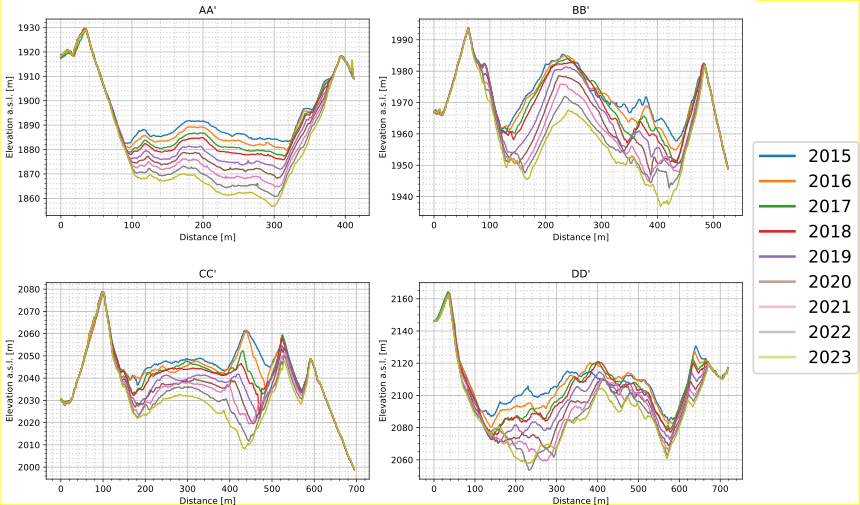
\includegraphics[width=\textwidth]{profiles.png}
  } \\
  \subcaptionbox{\label{fig:3:profiles:map}}{
    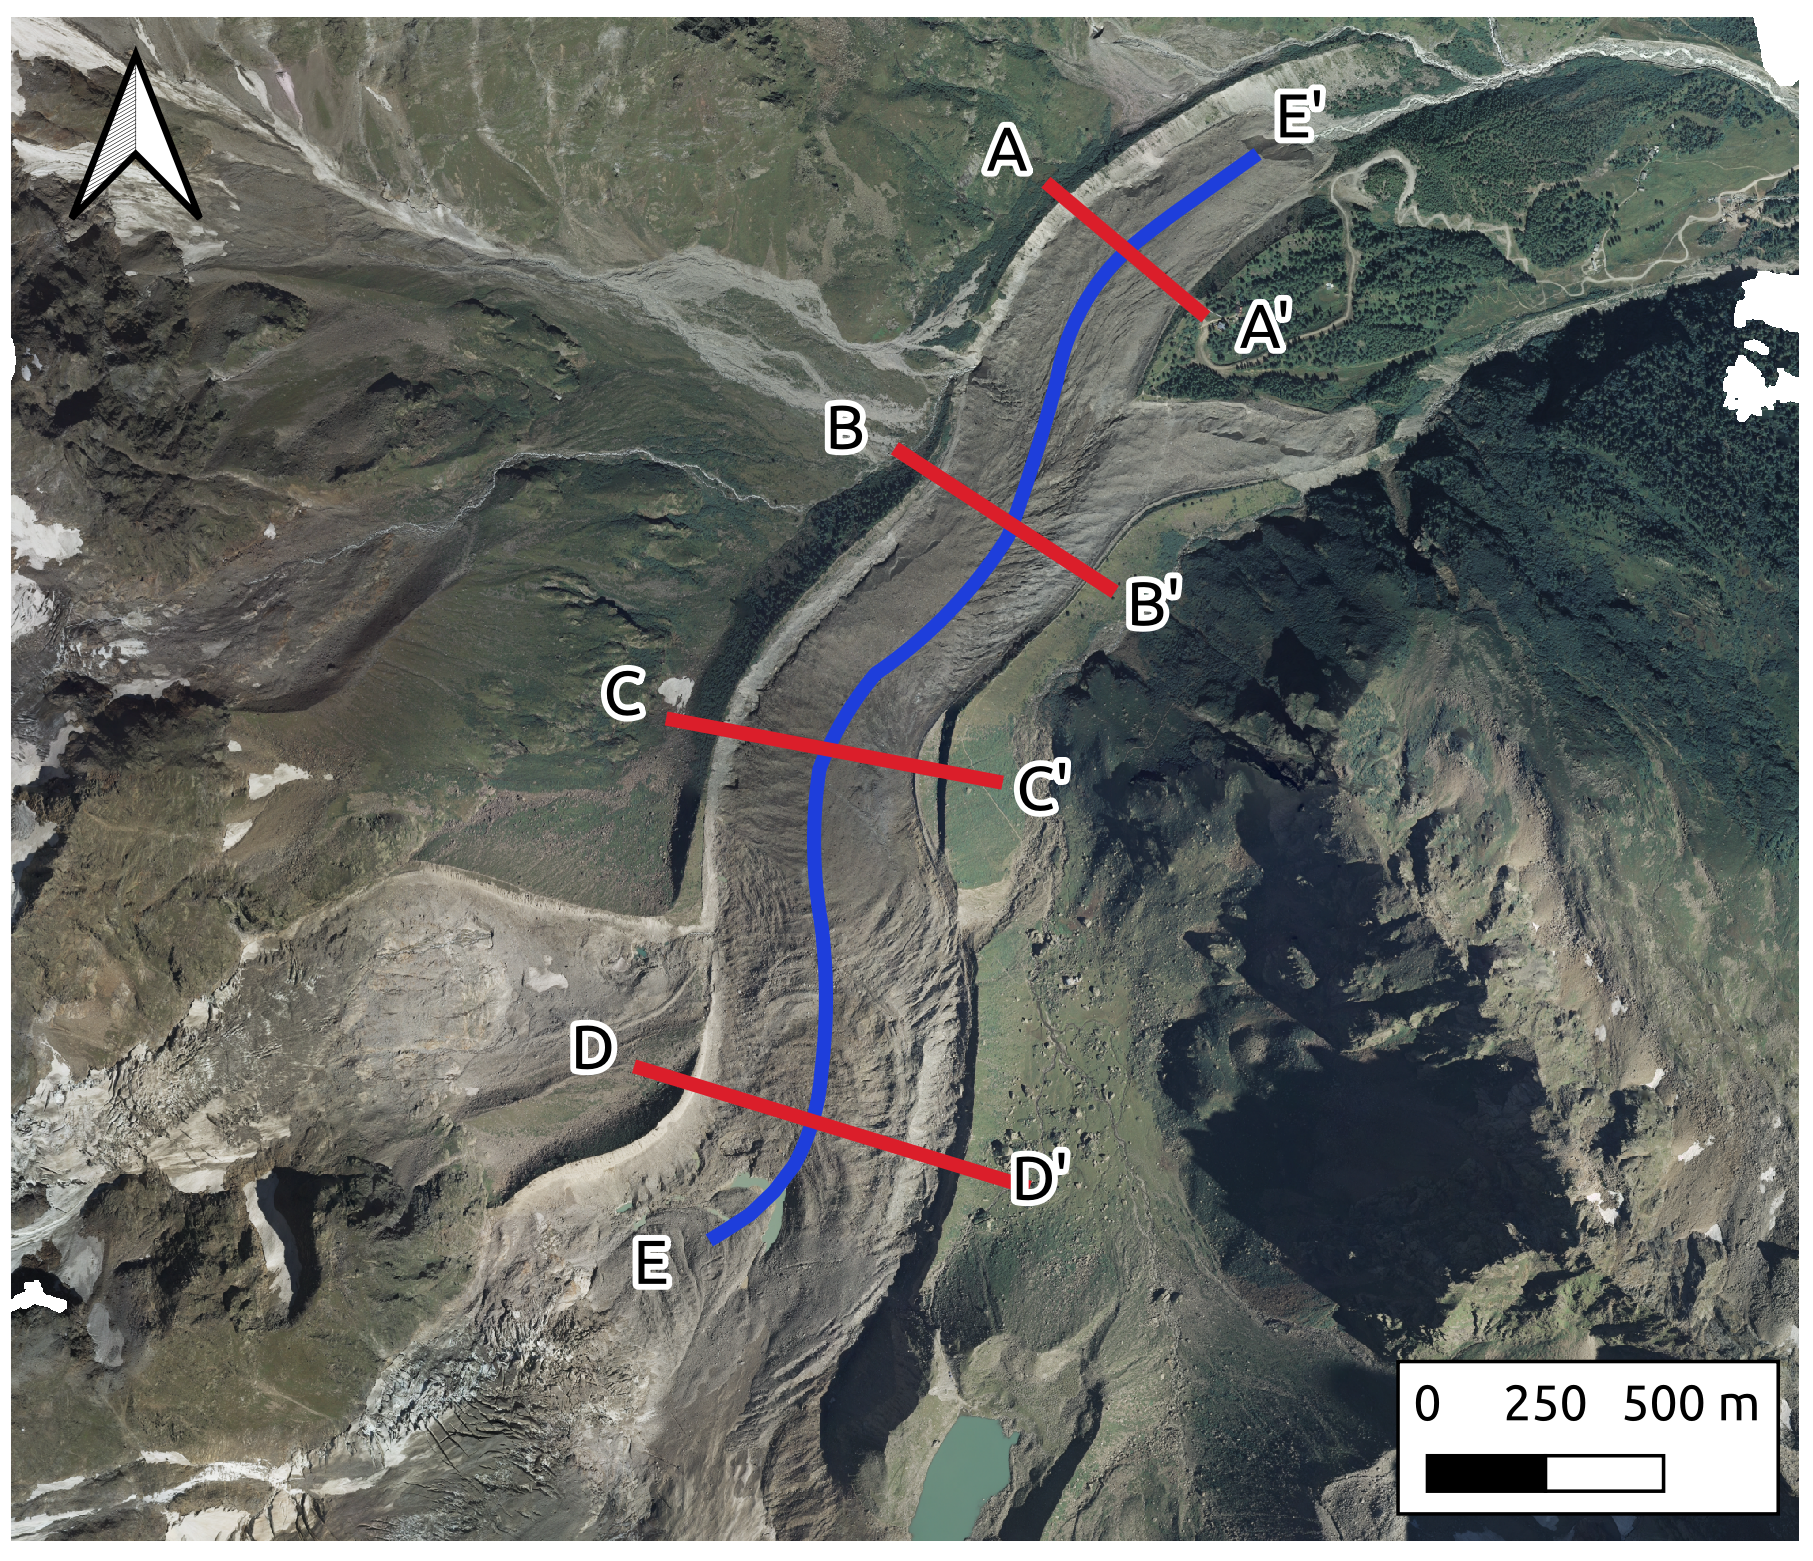
\includegraphics[width=.6\textwidth]{profiles_map.png}
  }
    \caption{\textbf{(a)} Elevation profiles obtained from the DSM computed for the years 2015-2023 along four different cross-sections. \textbf{(b)} Location of cross-sections. Cross-sections are viewed from south to north (i.e., from upstream to downstream of the glacier), as indicated by the letters in \textbf{(e)}.}
    \label{fig:3:profiles}
\end{figure}

\begin{figure}[ht]
  \centering
  \includegraphics[width=\textwidth]{longitudinal_profiles.png}
  \caption{Longitudinal profiles of the glacier extracted each year along the centerline. The location of the profile is marked in \figref{fig:3:profiles:map}.}
  \label{fig:3:profile_long}
\end{figure}

\figref{fig:3:volumes} depicts the year-on-year ice volume depletion, with error bars 
representing the estimated variance of volume variation. 

As the transition of fieldwork from Autumn to Summer in the period between 2017 and 2018 altered 
volume assessment timing, the volume loss for 2017--2018, computed from October 2017 to July 2018, 
primarily reflects wintertime and springtime variations.
Therefore it can not be directly compared with the annual average.
Moreover, ice volume loss for the period 2019--2020 might be marginally underestimated due to
significant geometric discrepancies in the photogrammetric model of the glacier's upper portion,
indicated by a larger Root Mean Square Error (RMSE) in the vertical direction (\SI{0.28}{\meter}, 
see \secref{sec:3:problems}), attributed to the absence of Ground Control Points (GCPs) measured 
in situ during photo acquisition. 

The ice volume variation observed from 2015 to 2023 reveals a striking and substantial trend, 
characterized by an average annual volume loss of \SI{3.21e6}{\cubic\meter} of ice. 
Excluding the period of 2017--2018, the year with the least ice depletion occurred between 2015 and 2016,
amounting to \SI{2.23e6}{\cubic\meter}. 
Conversely, the exceptionally hot and dry summer of 2022 left a significant mark, resulting in a notable volume 
loss of \SI{4.90e6}{\cubic\meter} during the period of 2022--2023.
The increasing trend in ice volume loss underscores the sensitivity of glacier systems to climatic variations and 
emphasizes the need for continued monitoring and analysis to comprehend the evolving dynamics of glacial environments.
These findings align with those observed in other alpine glaciers, such as the Mont Blanc glaciers~\citep{Berthier2023b_exceptional_thinning}.

In \figref{fig:3:profiles}, elevation profiles of the glacier obtained annually at four distinct cross sections are depicted collectively. 
Each profile delineates the glacier surface, demarcated by the lateral moraines. 
The series of cross-section AA' extracted at the northern terminal lobe (\figref{fig:3:profiles}a) shows a regular decrease in the glacier thickness
ice loss rate of approximately \qty{2}{\meter\per\year}.
In the other sections situated in the central and upper parts of the glacier (sections BB', CC', and DD', \figref{fig:3:profiles}b-d), 
the height reduction displays less regularity owing to the presence of crevasses.

Moreover, the formation of local peaks and valleys within the debris, arising from locally different melting processes, significantly disrupts the glacier's transfer zone. 
These features are particularly noticeable in the cross-sections BB' and DD'.
Notably, the streamwise right moraine of the glacier experiences progressive sliding processes and collapses due to the diminishing support of the thinning glacier. 
This phenomenon is prominently observed in both section AA' and section DD'.

\section{Glacier volumes variations from 1977 to 2023}

By integrating historical aerial surveys (Chapter \ref{ch:2}) with repeated in-situ UAV measurements, this study quantified long-term cumulative volume variations in the Belvedere Glacier (\figref{fig:3:cumulative_volumes_mass:volumes}).
For periods exceeding 5 years, an average ice density of\SI[separate-uncertainty = true]{850 \pm 60}{\kilo\gram\per\cubic\meter} was used to convert volume variations into mass changes \cite{Huss2013_density_geodetic_balance}. 
However, recognizing the limitations of this assumption for shorter periods (< 3 years) due to potential density variations \cite{Huss2013_density_geodetic_balance}, the analysis focused specifically on three surveys (2015, 2019, 2023) spaced by approximately 5 years. 
Volume variations between these surveys were calculated using a DOD approach and subsequently converted into ice mass variations  (\figref{fig:3:cumulative_volumes_mass:mass}). 
This strategy mitigates the uncertainty associated with density assumptions for short-term mass balance assessments.

\begin{figure}
  \centering
    \subcaptionbox{\label{fig:3:cumulative_volumes_mass:volumes}}{
    \includegraphics[width=0.8\textwidth]{cumulative_volume_variations_all.png}
  } \\
  \subcaptionbox{\label{fig:3:cumulative_volumes_mass:mass}}{
    \includegraphics[width=.8\textwidth]{cumulative_mass_changes_all.png}
  }
    \caption{(a) Cumulative volumes variations Belvedere Glacier (1977-2023) with 1977 as the reference year (b) Cumulative ice mass variations (in megatonnes), assuming an ice density of \SI[separate-uncertainty = true]{850 \pm 60}{\kilo\gram\per\cubic\meter}, considering periods longer than 5 years \cite{Huss2013_density_geodetic_balance}. \textcolor{red}{Make again computation volume differences for period 2015-2023}} 
  \label{fig:3:cumulative_volumes_mass}
\end{figure}

The Belvedere Glacier experienced increasing mass from 1977 to 2001, highlighting that the Belvedere Glacier was still experiencing an expansion. 
This trend abruptly ended with the 2000-2002 surge event, resulting in a significant mass gain around 2001. 
Subsequently, the glacier has undergone a continuous and dramatic retreat. 
As of 2023, the Belvedere Glacier has lost \SI{\sim 24}{\mega\tonne} of ice mass compared to its 1977 state.

\section{An open-source framework for sharing monitoring results}\label{sec:3:open-data}

A long-term monitoring campaign of Belvedere Glacier has produced a rich dataset that includes high-accuracy in-situ GNSS measurements, 3D point clouds, digital surface models (DSMs), and orthophotos derived from UAV photogrammetry.
In recognition of the value of collaboration and open science, all point clouds, DSMs, and orthophotos for the entire glacier have been made publicly available under the GNU General Public License (GPL) version 3 license through a Zenodo repository\footnote{\url{https://doi.org/10.5281/zenodo.7842347}}~\citep{ioli_2023_zenodo}.
This open-access initiative encourages further scientific exploration and evaluation by researchers across disciplines.
This will allow replication of the analyses performed in this thesis, such as estimates of glacier velocity and volume change, and facilitate the study of geomorphological processes such as moraine collapse and derive new insights into glacier dynamics. 
All data are accompanied by a structured JSON file containing essential metadata, allowing researchers to easily use the data for their purposes.

To maximize accessibility also for non-expert users, the 3D point clouds derived from all the surveys were converted to a Potree-compatible structure~\citep{schutz2016potree} and uploaded to a web server.
Potree is an open-source WebGL-based JavaScript library designed for web-based rendering of large-point 
clouds and it offers versatile tools for handling 2D and 3D objects, scene navigation, and interaction, including measurements and cross-section profile extraction~\citep{Gaspari2024, Fascia2024}.
The 3D glacier models are accessible from any web browser (\figref{fig:3:potree}), allowing users to navigate through different years and experience the evolution of the glacier over time\footnote{\label{the-belvedere-glacier-website}\url{https://thebelvedereglacier.it/potree/index.php}}.
\marginpar[Note 1]{
    \includegraphics[width=\marginparwidth]{qr_thebelvedereglacier.png}
}

\begin{figure}[p]
  \centering
    \subcaptionbox{\label{fig:3:profiles:potree:viewer}}{
    \includegraphics[width=0.95\textwidth]{potree_viewer.png}
  } \\
  \subcaptionbox{\label{fig:3:profiles:potree:sections}}{
    \includegraphics[width=.95\textwidth]{potree_sections.png}
  }
    \caption{\textbf{(a)} Web platform based on Potree for exploring the photogrammetric point clouds of the Belvedere Glacier acquired during the different surveys. \textbf{(b)} Example of two cross sections extracted directly from the Potree web interface from the point clouds of 2023 and 2015 to easily estimate the glacier thinning.}
    \label{fig:3:potree}
\end{figure}

Additionally, a robust open-source relational database serves as the central repository for the outcomes of the monitoring campaign, ensuring easy storage, use, and sharing. 
We chose PostgreSQL for its flexibility, permissive open-source license, and ability to manage geospatial data through the PostGIS extension seamlessly. 
This integration allows direct use within GIS software packages such as QGIS. 
Using a database centralizes data storage and provides remote access while allowing customizable permission levels. 
This allows public access (e.g. via a read-only web interface) while protecting sensitive data for internal use. 

The database primarily serves as a repository for field survey data, including details such as survey dates, instrument specifications, key acquisition parameters, and selected processing statistics. 
It also contains periodic GNSS measurements of photogrammetric targets and outputs from photogrammetric processes, including DSMs, orthophotos, derived glacier velocities, and volume changes.

\begin{figure}[ht!]
  \centering
  \includegraphics[width=0.9\textwidth]{belvederedb_erd.png}
  \caption{ERD diagram of the PostgreSQL database used for storing the Belvedere results. \textcolor{red}{Update fig}}
  \label{fig:3:belvederedb_erd}
\end{figure}

Following the principles of relational databases, data is structured across multiple tables, with access facilitated by defined relationships using primary and foreign keys. 
The logical model of the database, shown in \figref{fig:3:belvederedb_erd}, describes the main tables and their relationships.
Key components of the database include the \textit{surveys} table, which contains information about each survey; the \textit{points} table, which catalogs points that have been periodically GNSS surveyed; and the \textit{measurements} table, which contains the actual GNSS measured coordinates. 
Each measurement is associated with a survey record, which allows retrieval of survey timing and instrumentation information used to collect the measurement, and a point record, which associates the measurement with a specific point label, allowing tracking of points in time.
Each measurement can be associated with an image, stored in a separate table, to document the acquisition.
In the \textit{surveys} table, each survey is linked to its corresponding metadata stored in the \textit{instruments} table, which contains information on all instruments used over the years, and the \textit{flights} table, which contains details of each photogrammetric flight performed.
In addition, each survey is associated with the products derived from the photogrammetric processing.
This organizational structure streamlines data retrieval using SQL queries, enabling tasks such as extracting measurements from individual surveys or ranges of surveys and deriving displacement time series for specific points.

This structure defines the core of the database, which is intended for internal use. 
However, to improve accessibility and streamline data retrieval, a set of predefined queries has been used to create read-only views (i.e., read-only subsets of a database based on a query that runs on one or more tables) within a separate public schema. 
These views provide a higher level of abstraction, allowing easy access to all relevant information.
These views include functions such as accessing all measured points for each year, identifying active points (i.e., targets still present on the glacier and not lost) by providing their most recent measurement, and automatically calculating time series of displacements, velocities, and accelerations for each point by differentiating consecutive measurements.
Additional functionalities encompass the automatic conversion of GNSS coordinates from the geographic WGS84 reference system to the projected RDN2008 / UTM zone 32N reference system, and vice versa. Furthermore, the database facilitates the computation of orthometric heights for each measurement via bilinear interpolation using the Italian Geoid model ITALGEO05~\citep{Barzaghi2007}.

The database currently stores 456 GNSS measurements from 85 distinct points obtained across 19 surveys. 
The data can be conveniently accessed through GIS software like QGIS, made possible by the PostGIS database extension. 
This setup enables automatic plotting of points associated with each measurement on a map canvas, together with pre-defined visualization styles, facilitating visual analysis.
Furthermore, both researchers and non-expert users can access the public schema of the database via a dedicated web platform\footnote{\url{https://thebelvedereglacier.it}}. Here, users can effortlessly view the GNSS measurements on a web-map, extract time-series information, and download them for their scientific inquiries. 
Combining this with a web-based visualization of the 3D point clouds with Potree~\citep{schutz2016potree} makes it possible to have a complete overview of the outcomes of the Belvedere Glacier monitoring campaign.
This initiative not only promotes transparency and reproducibility in research but also cultivates collaboration and knowledge exchange within the scientific community.

\begin{figure}[ht]
  \centering
  \includegraphics[width=0.8\textwidth]{db_qgis_query.png}
    \caption{Example of georeferenced layer queries from the PostgreSQL database using QGIS. The layer symbology is directly stored within the database and is automatically loaded into the QGIS project upon layer loading.}  \label{fig:3:db_qgis_query}
\end{figure}

% References
\makechapterbibliography{}

